\section{Experiments Completed/Scheduled}   \label{sec:experiments}
% Experiments

In order to validate the position control approach proposed in section \ref{sec:technical-approach}, we conduct experiments on two parallel soft actuator systems. The first consists of three actuators constrained to 2 DOF motion (Figure \ref{fig:modules}a). The second consists of four actuators constrained 3 DOF motion (Figure \ref{fig:modules}b). 
    So far, all of our experiments have been conducted using the three actuator system.

During the experiments, the pressures inside the actuators are varied using pneumatic pressure regulars (Enfield TR-010-g10-s), and the displacement of the end effector is measured using a motion capture system (Phase Space Impulse X2E).

%% figure: the 2dor and 3dof modules, labeled, side to side
\begin{figure}
    \centering
    \begin{tikzpicture}
        \def\colWidth{0.4\linewidth}
        \matrix [row sep=0.5cm, column sep=1cm, style={align=center}] (my matrix) at (0,0)
        {
        \node[style={anchor=center}] {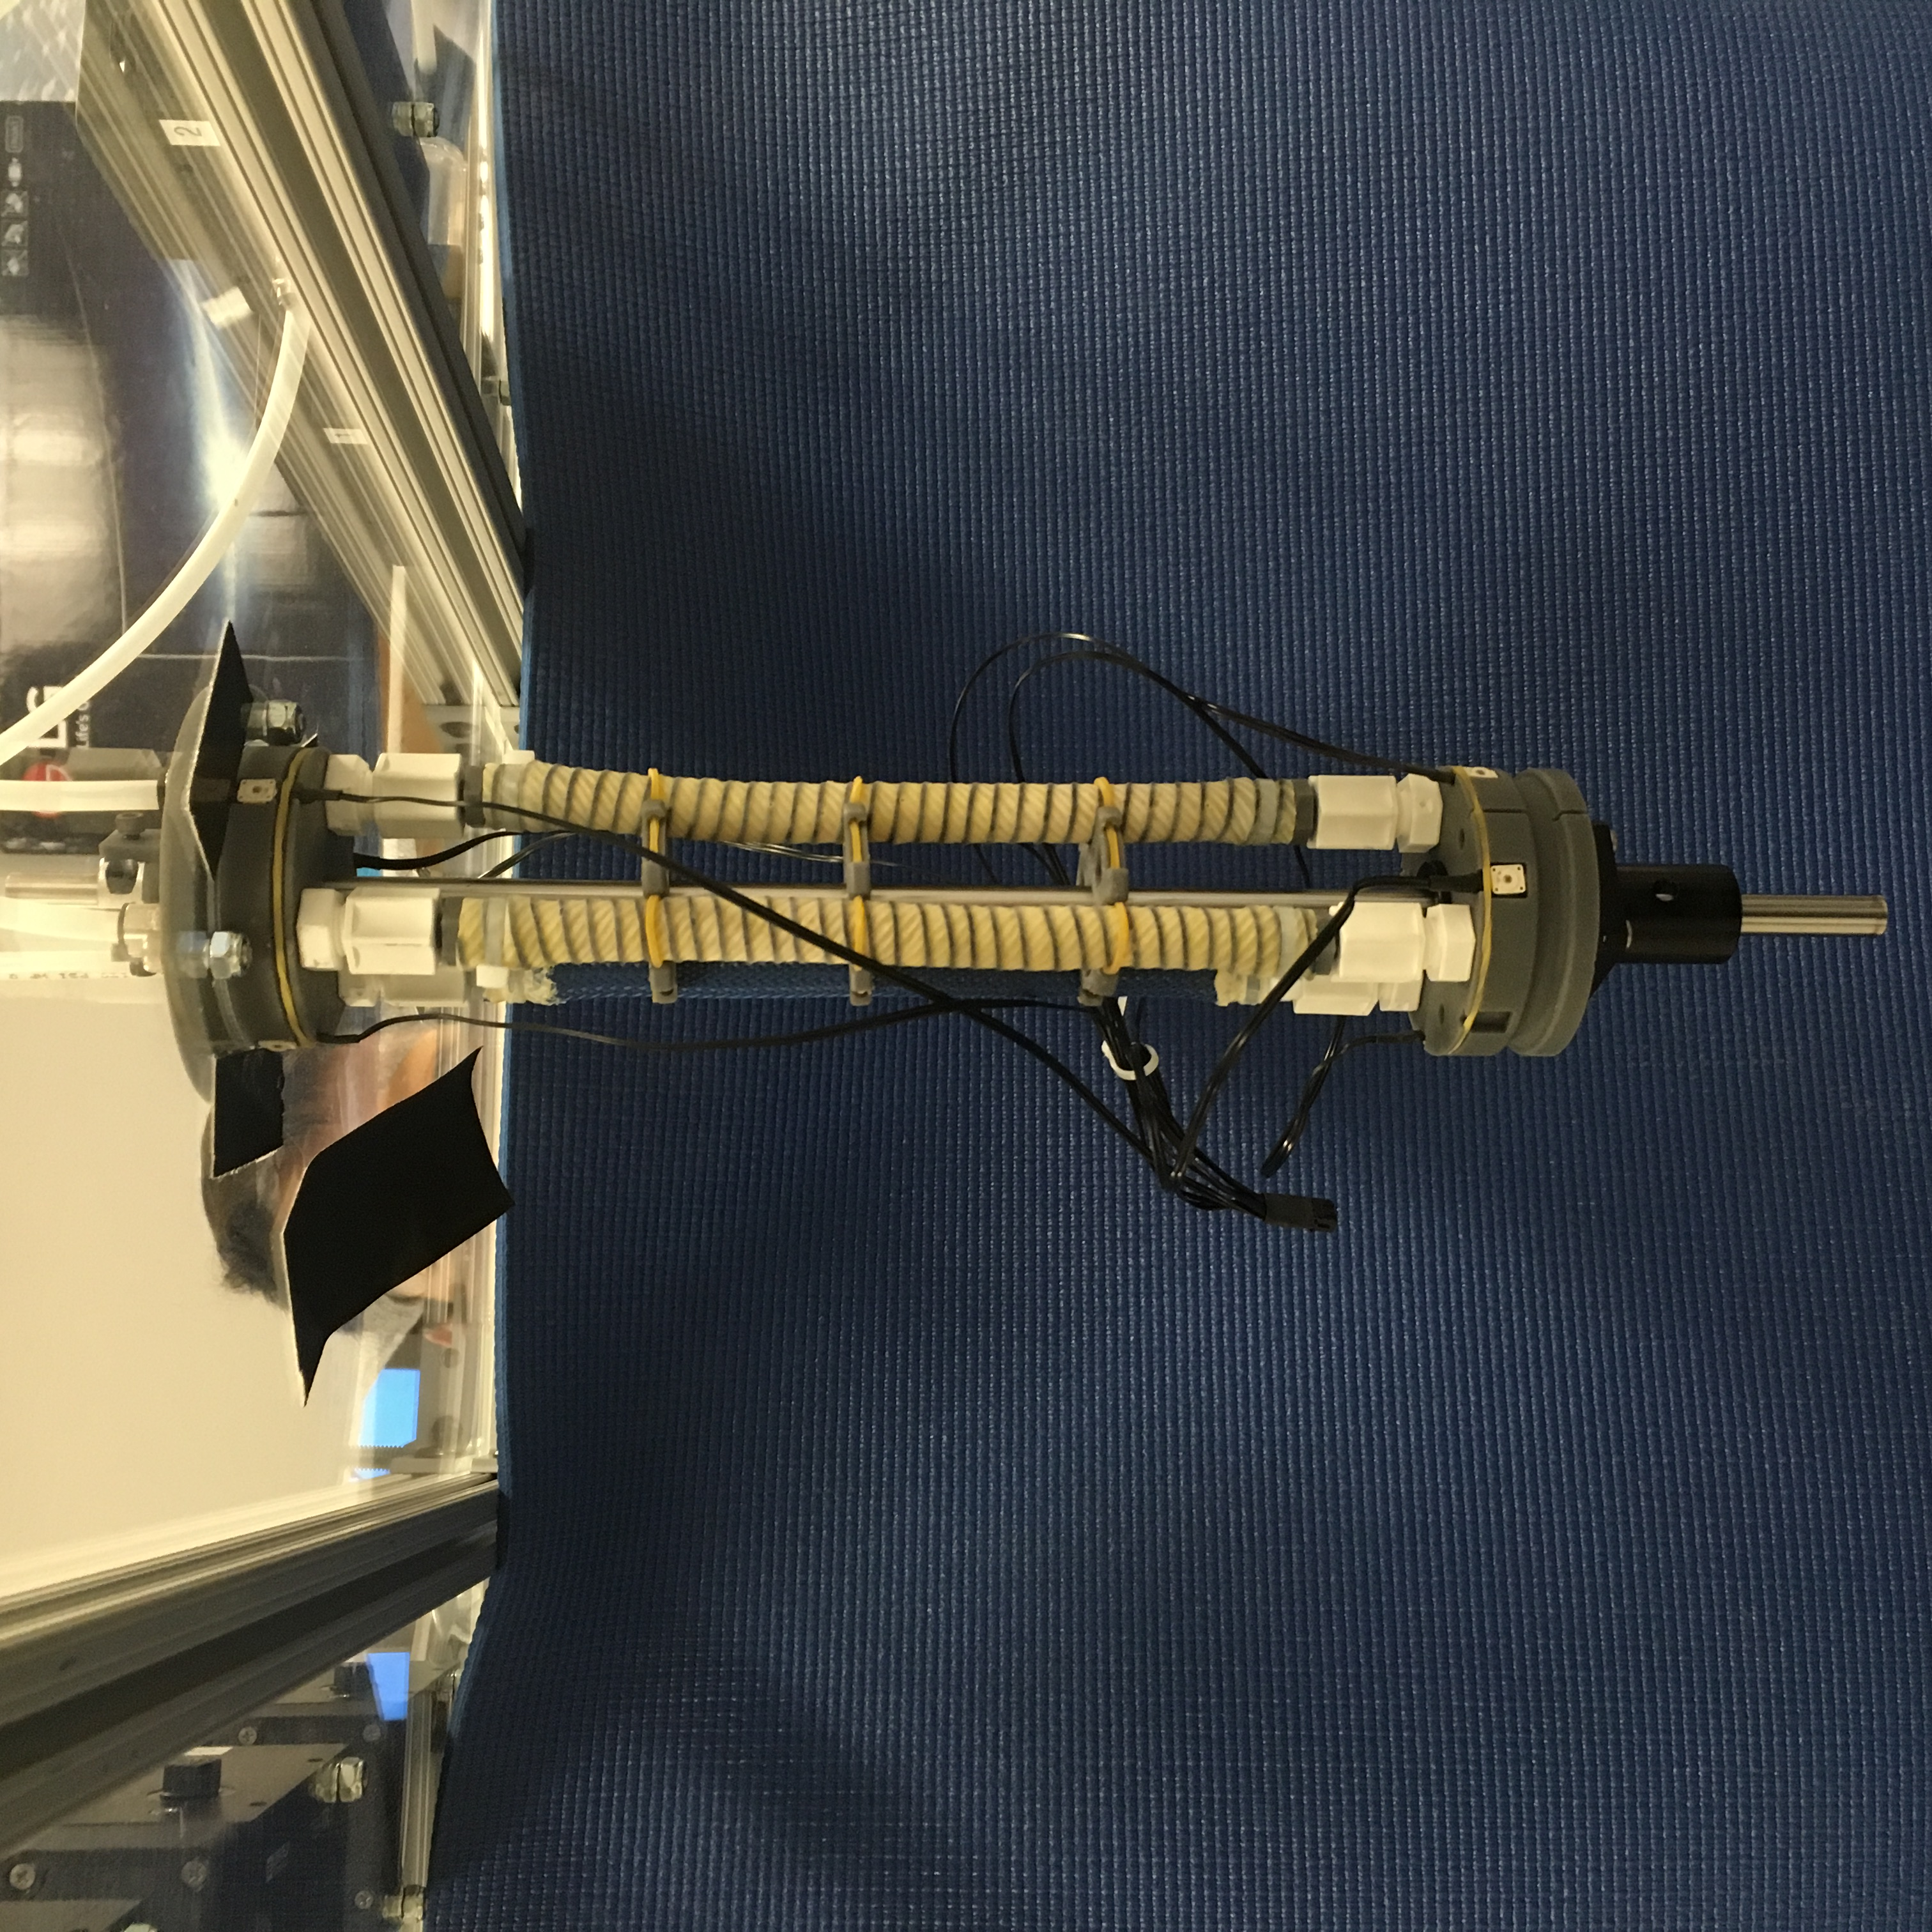
\includegraphics[width=\colWidth, angle=-90]{figures/free3.JPG}};
        &
        \node[style={anchor=center}] {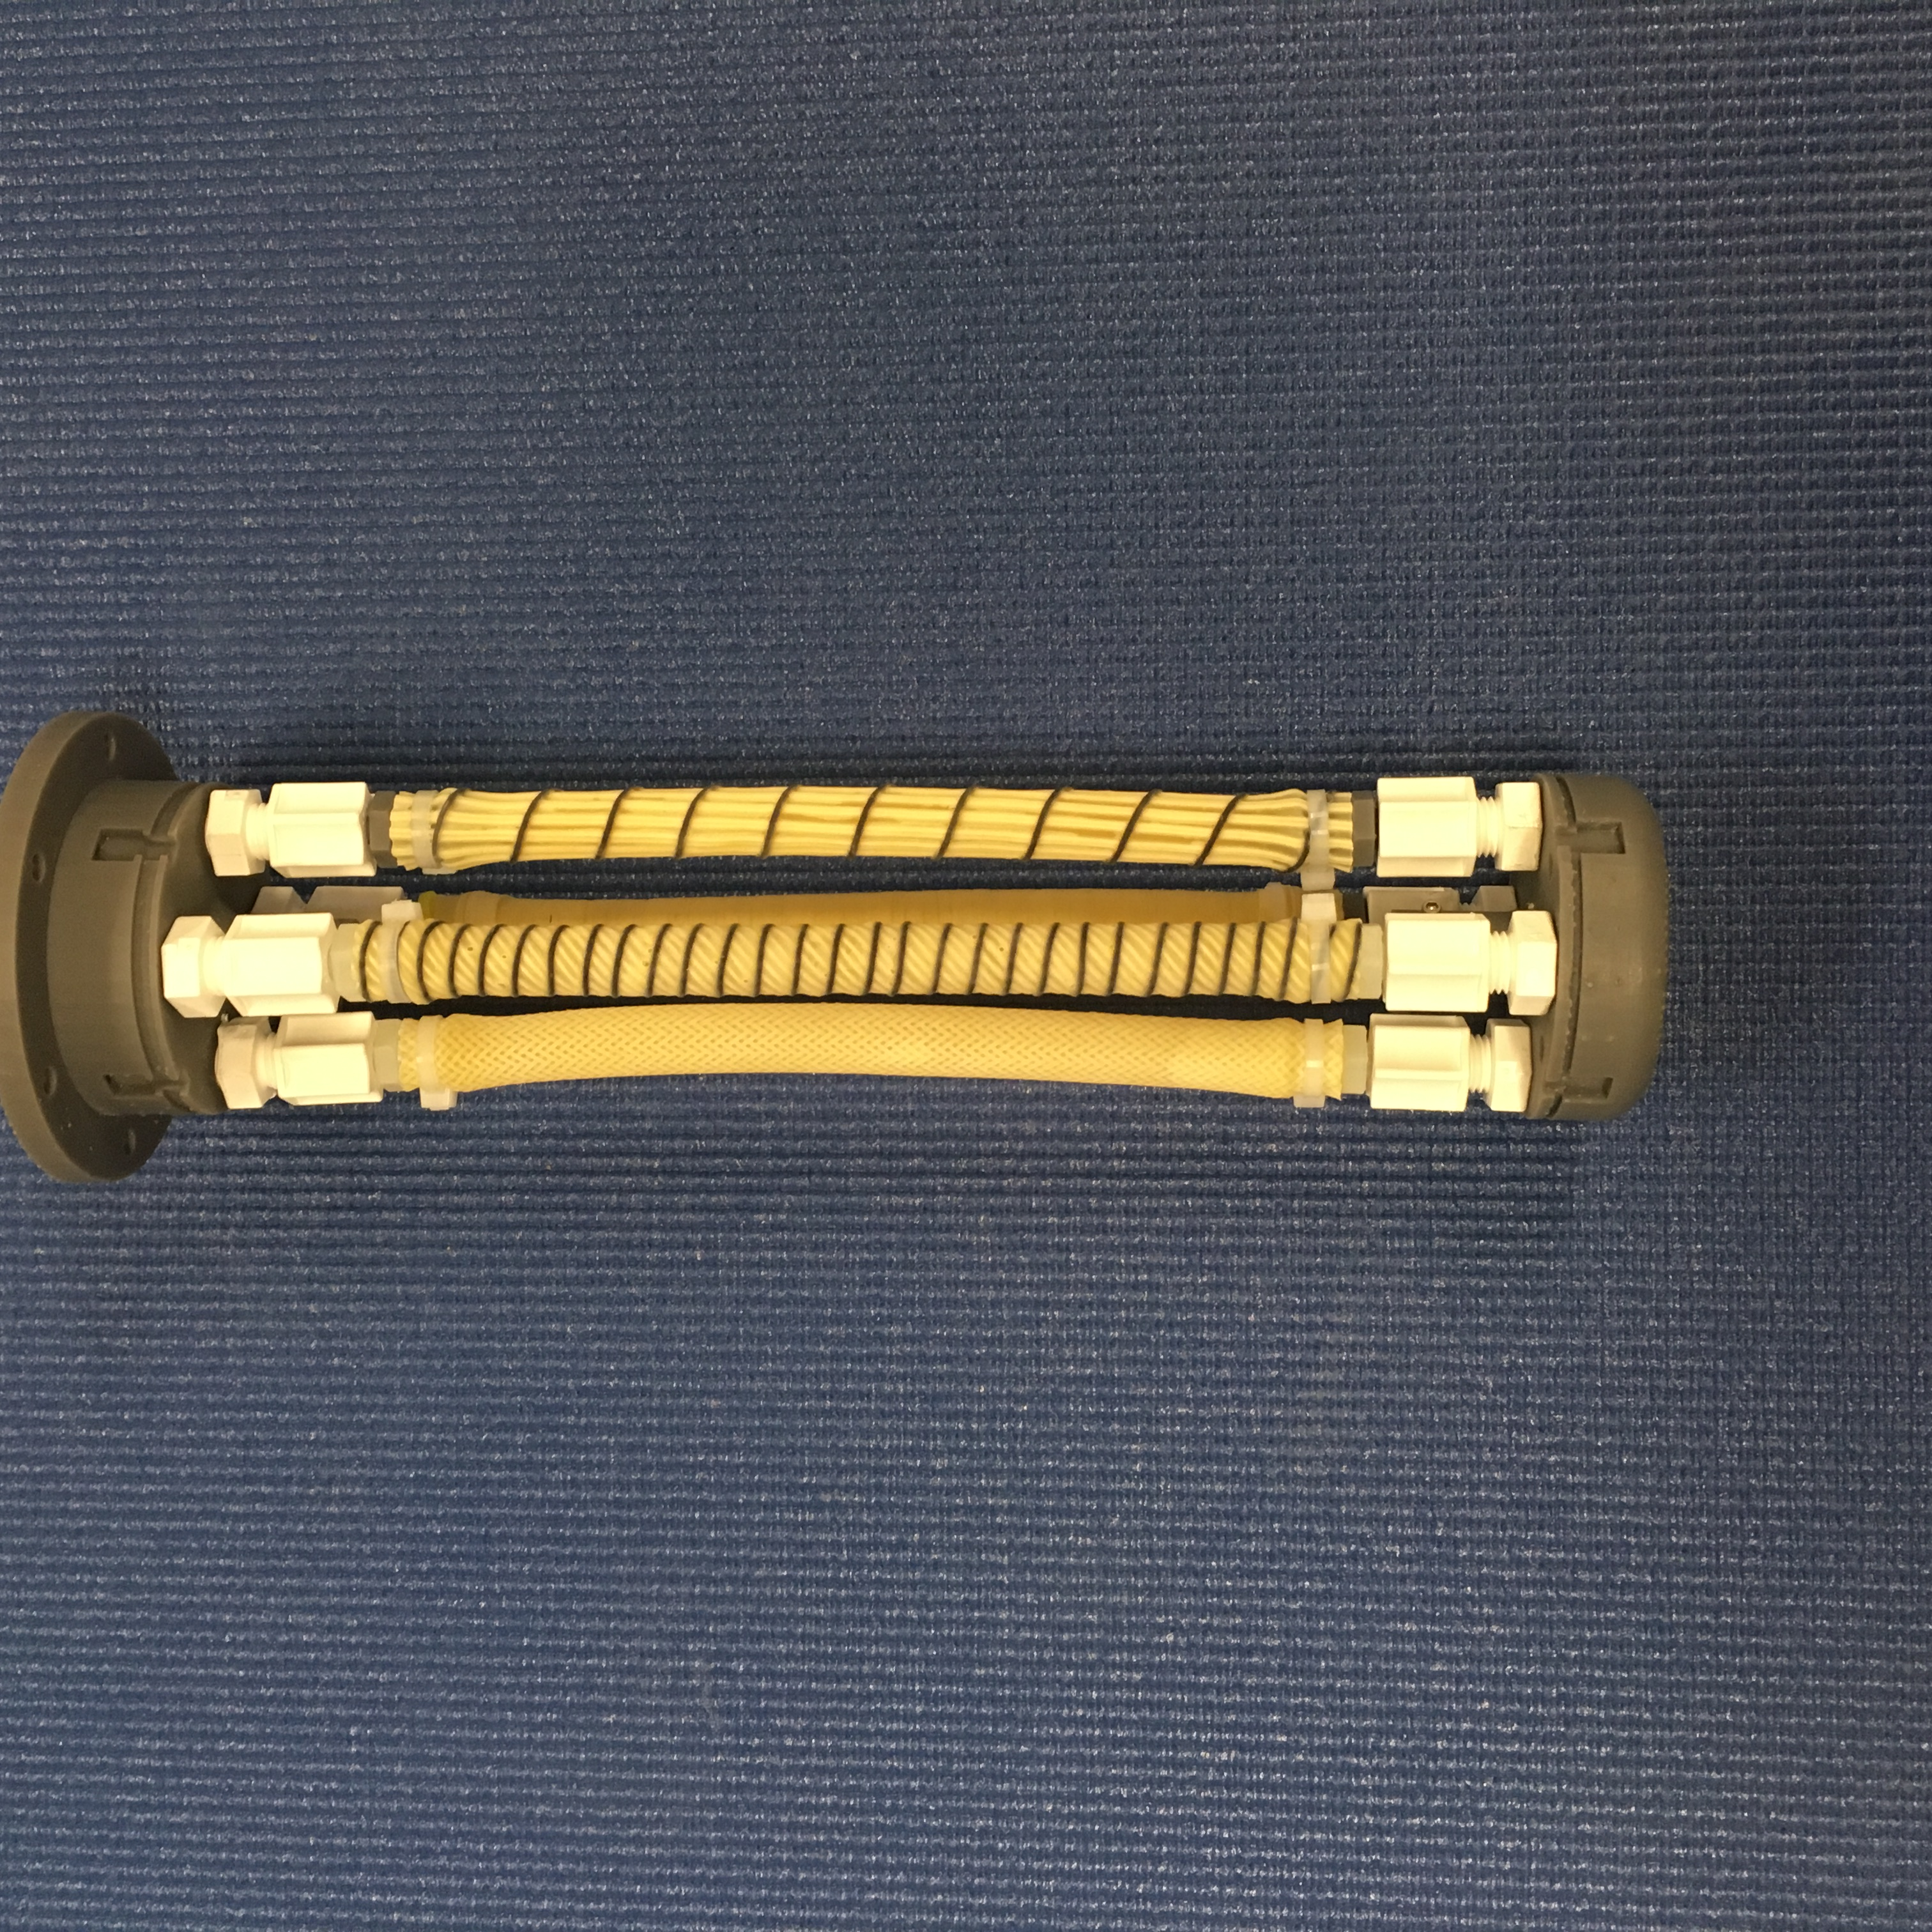
\includegraphics[width=\colWidth, angle=-90]{figures/free4.JPG}};
        \\
        };
    \end{tikzpicture}
    \caption{(a) A parallel system consisting of three FREE actuators attached to an end effector that is constrained to 2 DOF motion. A linear/rotary ball bearing allows the end effector to translate and rotate about a central shaft, while restricting motion in all other directions. (b) A parallel system consisting of four FREE actuators attached to an end effector that is constrained to 3 DOF motion. A centrally mounted spring-steel shaft  constrains the end effector to move on a 2D sub-manifold of 3D space, while also admitting rotations about its central axis. \Dan{these pictures/captions are placeholders. Will be replaced with much nicer versions with labels drawn on to show DOFs.}}
    \label{fig:modules}
\end{figure}

%% Experiments Completed



2DOF translation and rotation experiment. Iterate through a bunch of $\x^\tx{des}$ and compare the measured displacement to that predicted by the model, $\vec{e}_i = \x^\tx{des}_i - \x^\tx{meas}_i$. Then, do the same thing with a torsional load applied. Then do the same thing with unknown loads, but have a feedback loop with a gain on the fload term.

%% figure: 2dof rig in motion capture system


%% Experiments Scheduled
In future experiments we will apply the same approach to the less constrained system shown in figure \ref{fig:modules}b.
